\documentclass[border=5pt]{standalone}
\usepackage{tikz}
\usepackage{amsmath}
\begin{document}
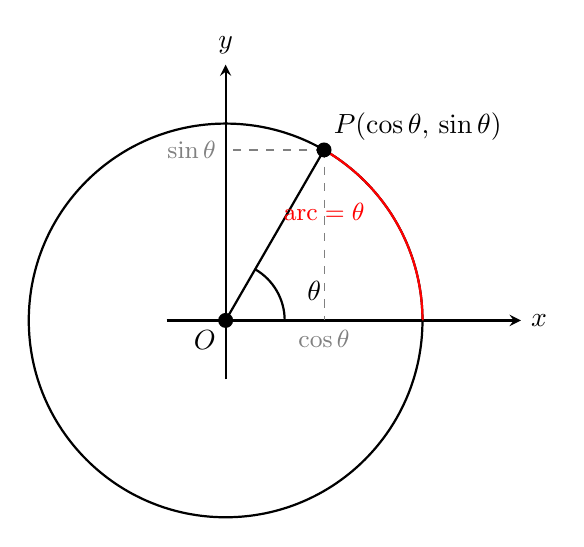
\begin{tikzpicture}[scale=2.5, >=stealth]
  % Unit circle
  \draw[thick] (0,0) circle (1);

  % Axes
  \draw[->, thick] (-0.3,0) -- (1.5,0) node[right] {$x$};
  \draw[->, thick] (0,-0.3) -- (0,1.3) node[above] {$y$};

  % Point P on circle at angle 60°
  \pgfmathsetmacro{\angle}{60}
  \pgfmathsetmacro{\px}{cos(\angle)}
  \pgfmathsetmacro{\py}{sin(\angle)}

  % Arc from (1,0) to P (highlighted in red)
  \draw[red, thick] (0:1) arc (0:\angle:1);

  % Lines from origin
  \draw[thick] (0,0) -- (1,0);
  \draw[thick] (0,0) -- (\px, \py);

  % Dashed projections
  \draw[dashed, gray, thin] (\px, \py) -- (\px, 0) node[below, font=\small] {$\cos\theta$};
  \draw[dashed, gray, thin] (\px, \py) -- (0, \py) node[left, font=\small] {$\sin\theta$};

  % Point P
  \filldraw[black] (\px, \py) circle (1pt) node[above right] {$P(\cos\theta,\, \sin\theta)$};

  % Origin
  \filldraw[black] (0,0) circle (1pt) node[below left] {$O$};

  % Angle arc
  \draw[thick] (0.3,0) arc (0:\angle:0.3);
  \node at (0.45, 0.15) {$\theta$};

  % Arc length label
  \node[red, font=\small] at (0.5, 0.55) {$\text{arc} = \theta$};
\end{tikzpicture}
\end{document}
